\section{Procedure}
\label{sec:Procedure}

The first step is to find the minimal current value for the laser setup, where
it is still lasing. For this measurement the setup is changed to the configuration shown in
figure~\ref{fig:setup_current}.
The minimum can be found in an iterative procedure, which follows the following
steps. First pick a current, where the laser is lasing.
Then lower the current slightly below the lasing threshold and try to bring the system back to lasing,
by adjusting the cavity with the two knobs.
If this is possible, lower the current
until it is slightly below the threshold and repeat the procedure.

\begin{figure}
  \vspace{-10pt}
  \centering
  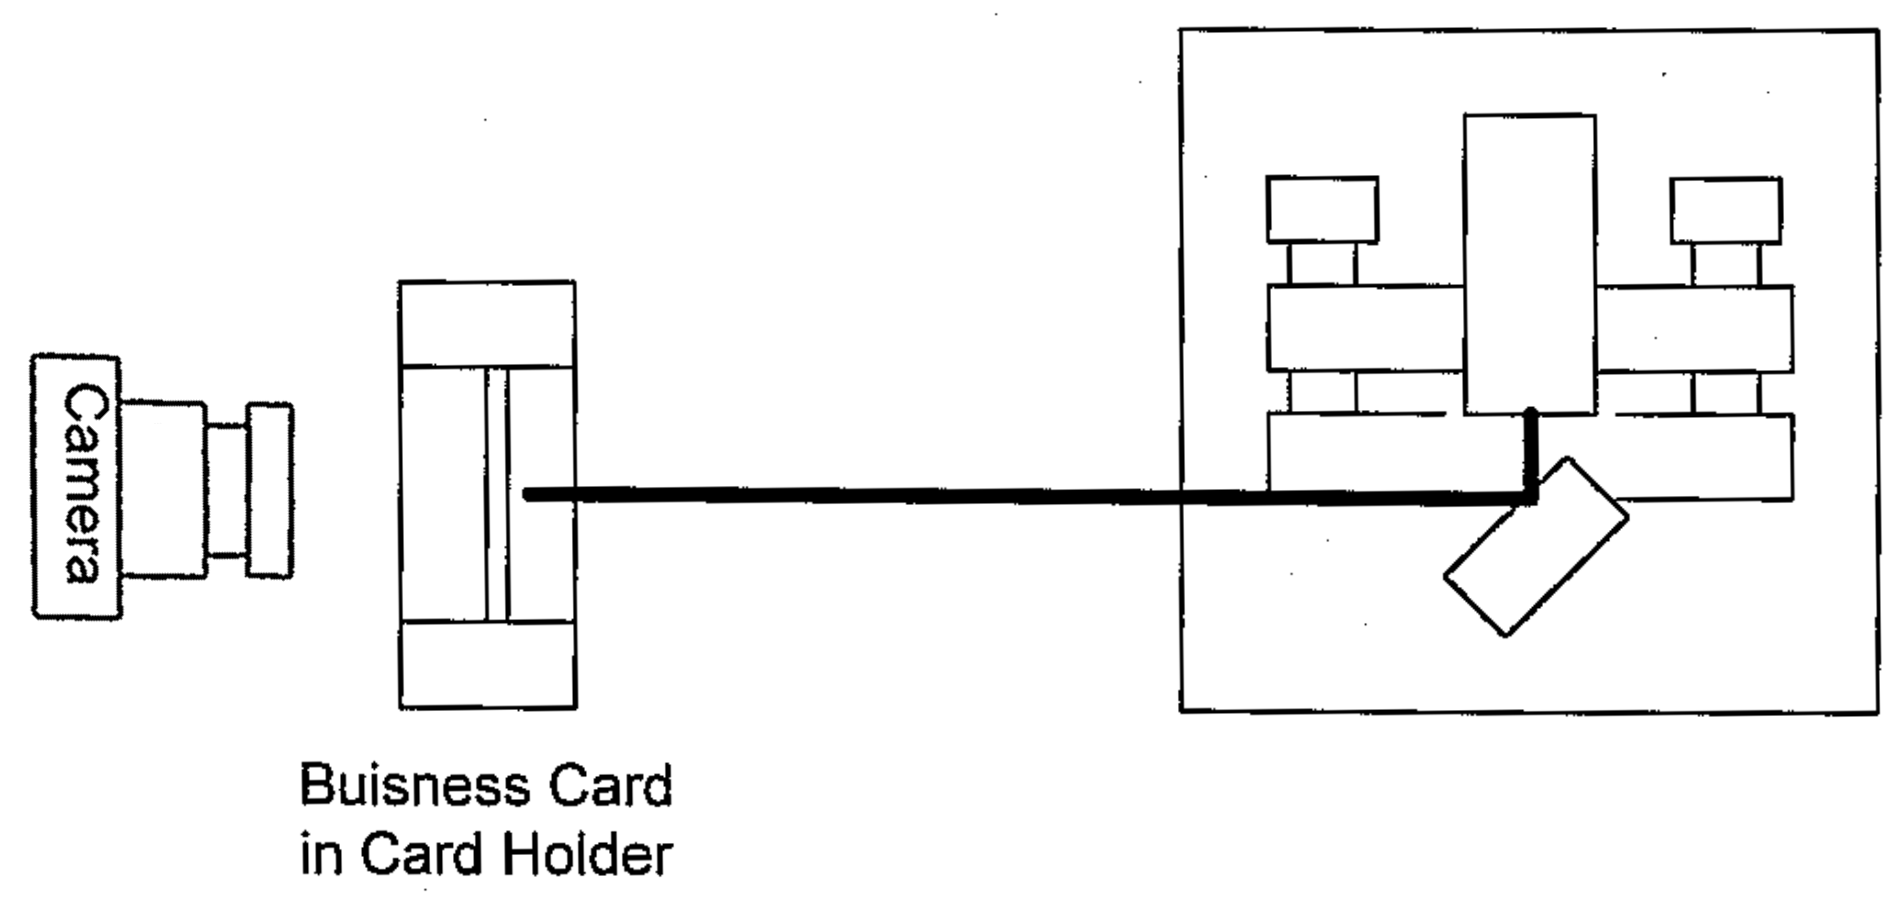
\includegraphics[width=0.8\textwidth]{Pics/setup_threshold.png}
  \caption{Setup for the minimum current measurement.\cite{anleitung}}
  \label{fig:setup_current}
\end{figure}

The minimun current below the threshold $I_{below}$ and the current above the treshold $I_{above}$
are given in~\eqref{eqn:nolase} and~\eqref{eqn:lase}.
The associated images of the laser spots are shown in figure~\ref{fig:no_lase}
and~\ref{fig:lase}.
\vspace{-10pt}
\begin{align}
  \label{eqn:nolase}
  I_{below} &= \SI{33.2}{\milli\ampere}\\
  \label{eqn:lase}
  I_{above} &= \SI{33.4}{\milli\ampere}
\end{align}

\begin{figure}[h!]
  \centering
  \begin{subfigure}{0.48\textwidth}
    \centering
    \includegraphics[width=\textwidth]{Pics/threshold_no_lase.jpg}
    \caption{Current below threshold $I_{below}$.}
    \label{fig:no_lase}
  \end{subfigure}
  \begin{subfigure}{0.48\textwidth}
    \centering
    \includegraphics[width=\textwidth]{Pics/threshold_lase.jpg}
    \caption{Current above threshold $I_{above}$.}
    \label{fig:lase}
  \end{subfigure}
\end{figure}
\FloatBarrier
The setup is now changed to the configuration, shown in figure~\ref{fig:setup_fluorescence}.
The image depicted in~\ref{fig:fluorescence} is than taken.

\begin{figure}
  \centering
  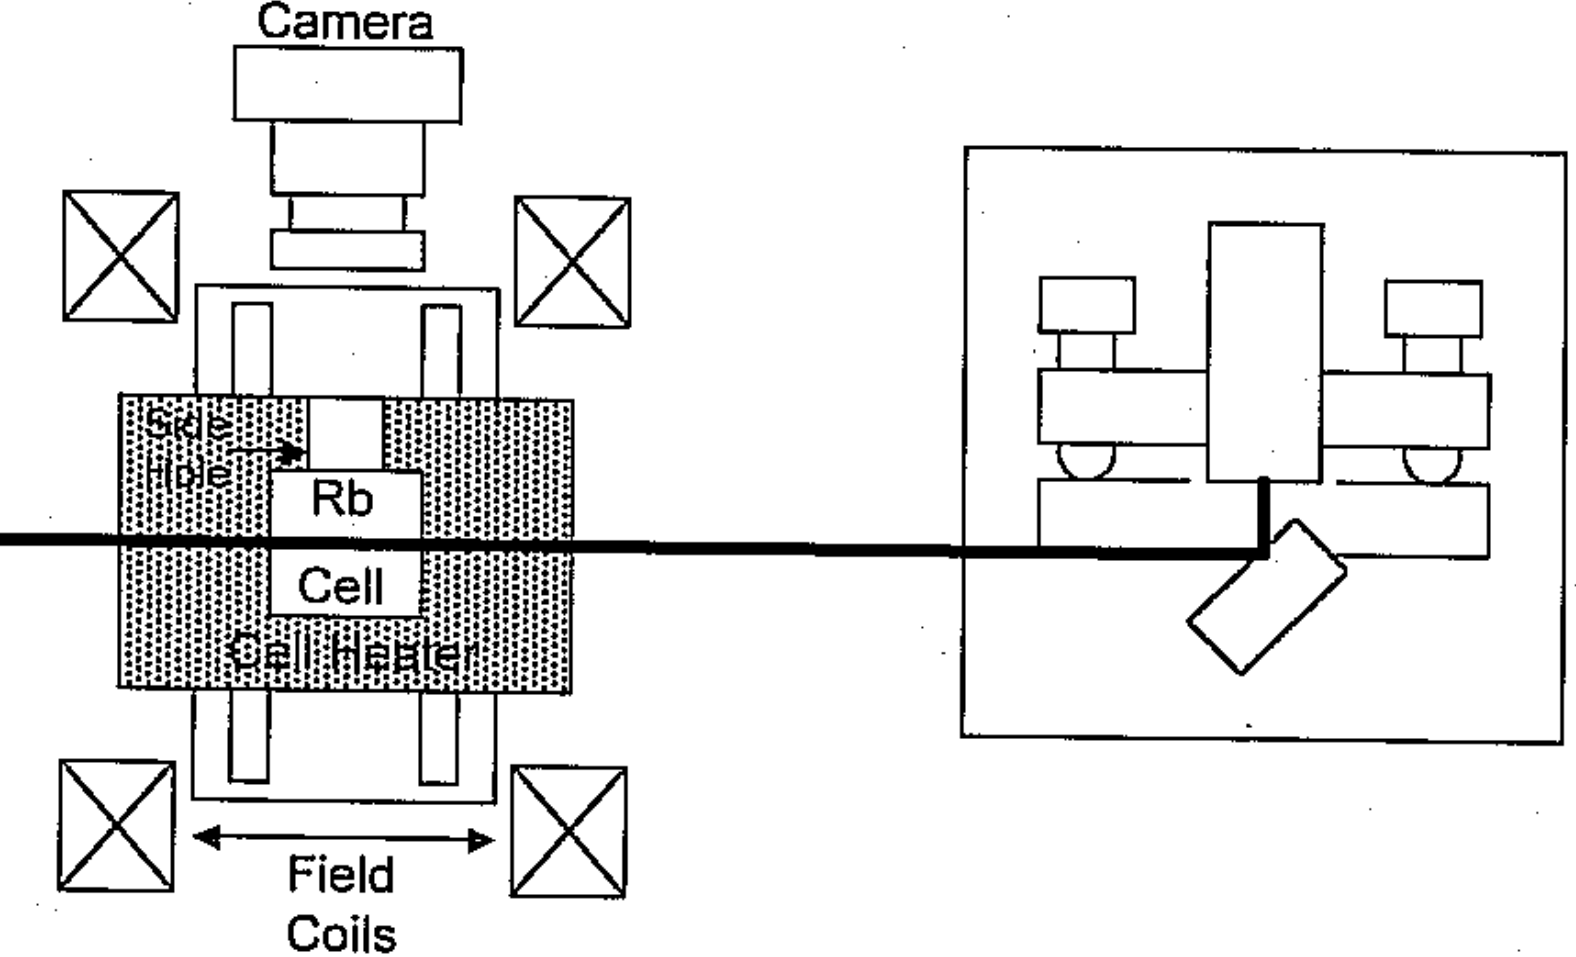
\includegraphics[width=0.8\textwidth]{Pics/setup_fluorescence.png}
  \caption{Setup to observe the Rubidium fluorescence line.\cite{anleitung}}
  \label{fig:setup_fluorescence}
\end{figure}

\begin{figure}
  \centering
  \includegraphics[width=0.5\textwidth]{Pics/Rb_fluorescence.jpg}
  \caption{Rubidium fluorescense line.}
  \label{fig:fluorescence}
\end{figure}



\begin{figure}
  \centering
  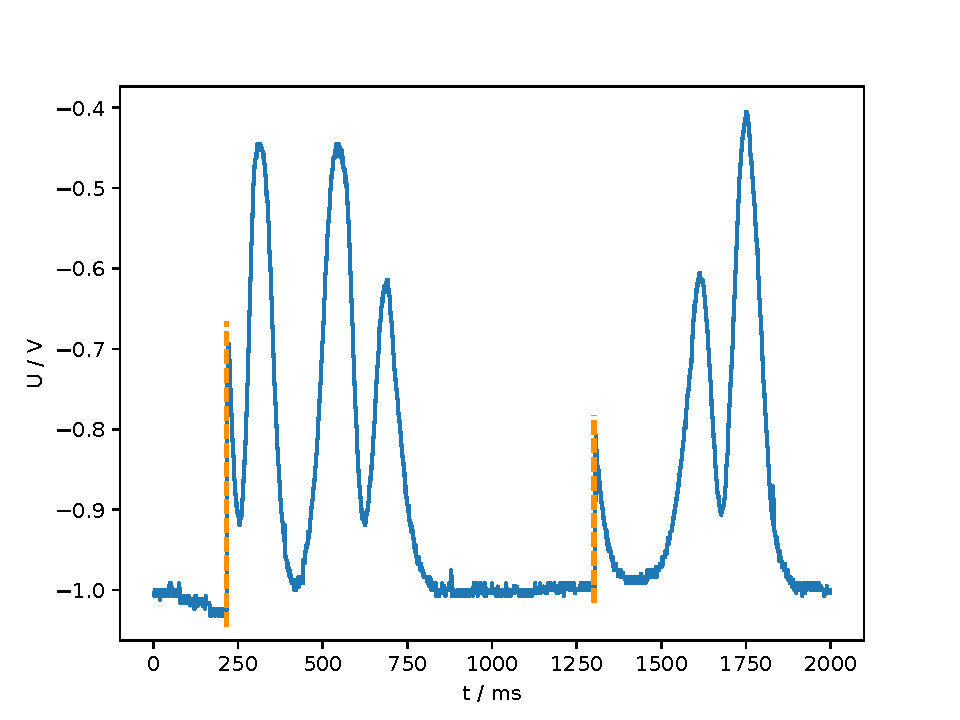
\includegraphics[width=0.7\textwidth]{Pics/example_spectrum_hop.pdf}
  \caption{Example spectrum. The mode hopes are indicated by the orange markers.}
  \label{fig:example}
\end{figure}

\begin{figure}
  \centering
  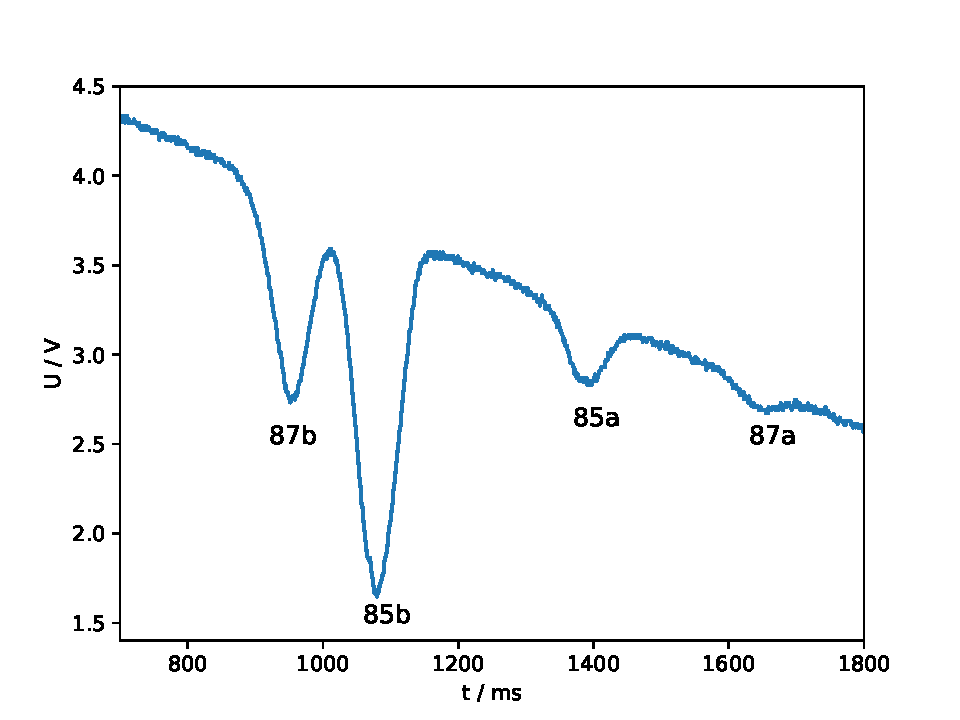
\includegraphics[width=0.7\textwidth]{Pics/Rb_spectrum.pdf}
  \caption{Rubidium spectrum.}
  \label{fig:spectrum}
\end{figure}

\begin{figure}
  \centering
  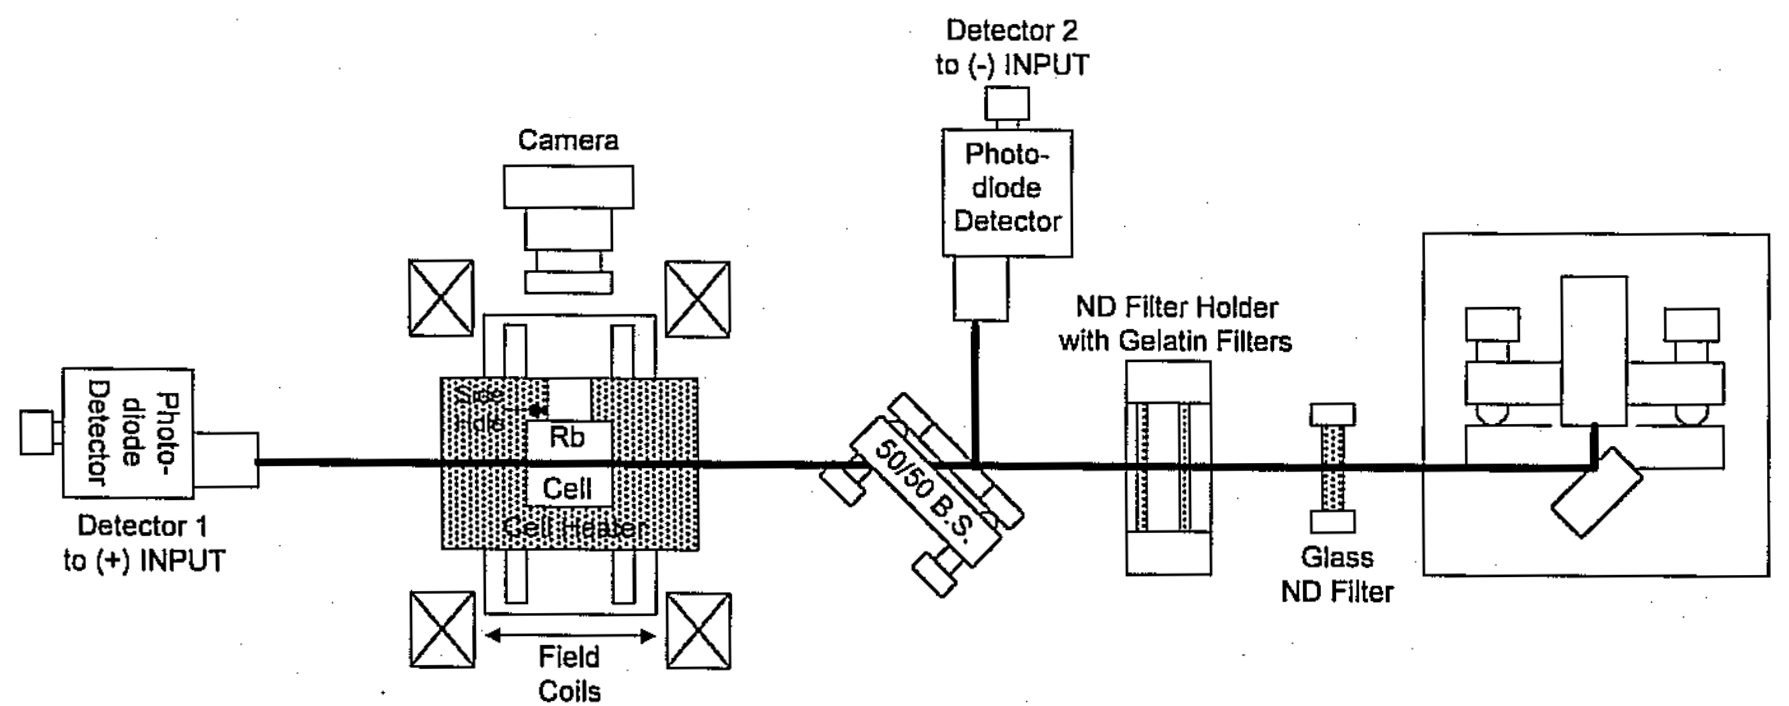
\includegraphics[width=\textwidth]{Pics/setup_substraction.png}
  \caption{Setup for the substraction technique measurement.\cite{anleitung}}
  \label{fig:setup_substraction}
\end{figure}

\begin{figure}
  \centering
  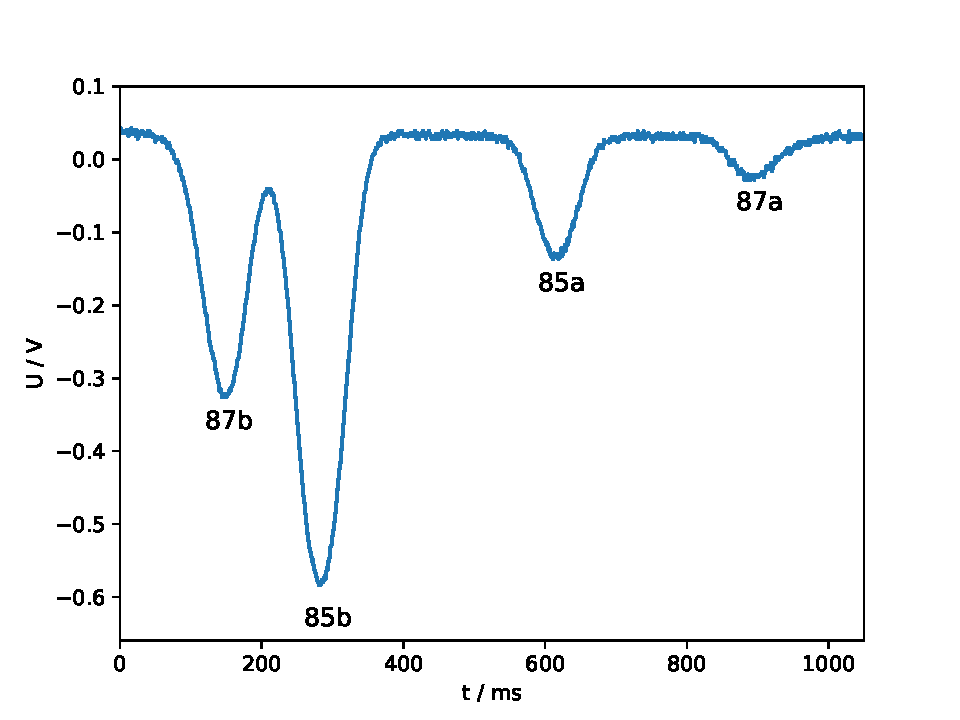
\includegraphics[width=0.7\textwidth]{Pics/Rb_spectrum_subst.pdf}
  \caption{Rubidium spectrum with substraction technique.}
  \label{fig:spectrum_sub}
\end{figure}
